% asset_id: FAS2RecurrenceRelationshipsTikZ-001
% asset_type: TikZ
% unit_code: FAS2
% topic_code: FAS2-REC
% topic_name: Recurrence relationships
% topic_id: FAS2RecurrenceRelationships
% lesson_file: FAS2_recurrence_relationships_lesson.md
% related_lesson_section: Section 9.7 Order and subscript diagram
% source: Transcript notation discussion
% purpose: Show indexed recurrence terms on a discrete index line and label first-order and second-order gaps.

\documentclass[tikz,border=8pt]{standalone}
\usepackage{amsmath}
\usepackage{xcolor}
\usetikzlibrary{arrows.meta,decorations.pathreplacing}
\definecolor{Canvas}{HTML}{FAF9F6}
\definecolor{Ivory}{HTML}{FFFFF0}
\definecolor{SoftPink}{HTML}{FBEFEF}
\definecolor{LineGrey}{HTML}{E5E5EA}
\definecolor{AccentGold}{HTML}{C5A059}
\definecolor{TextDark}{HTML}{2C2C2E}
\begin{document}
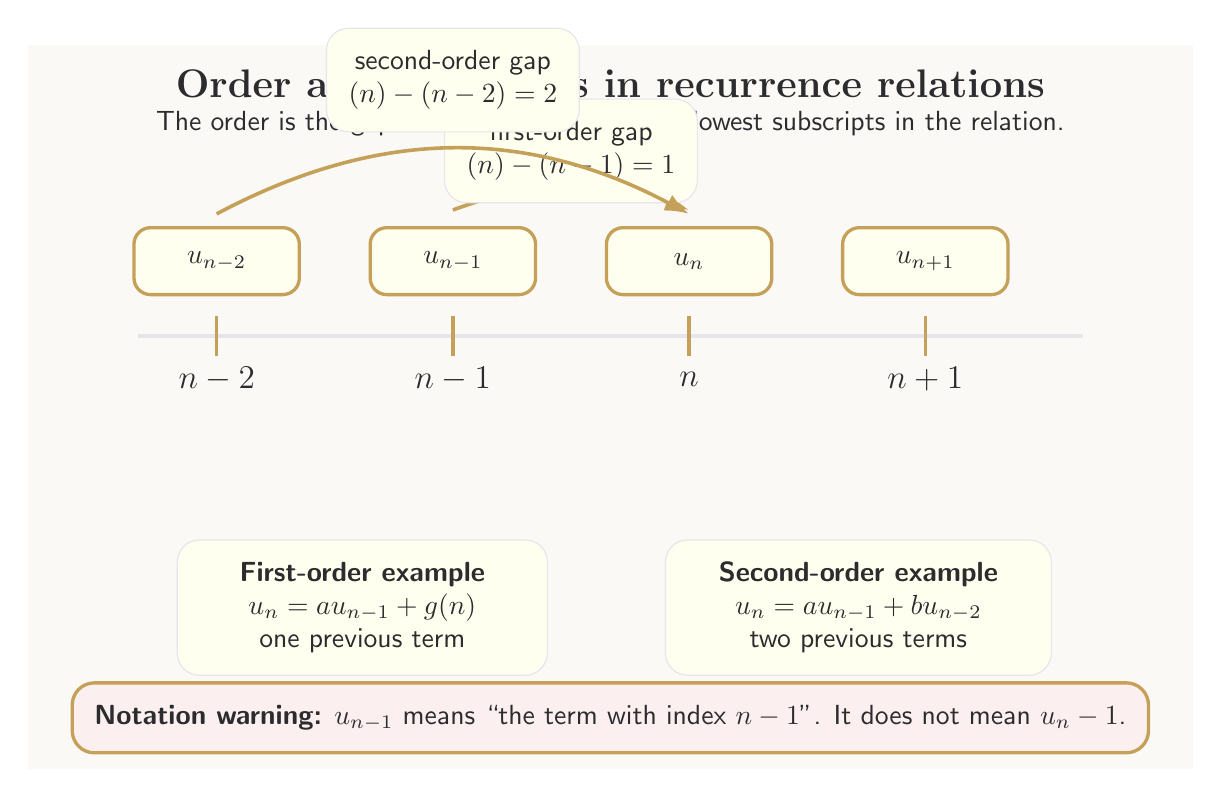
\begin{tikzpicture}[font=\sffamily,every node/.style={text=TextDark},arrow/.style={-{Latex[length=3mm]},draw=AccentGold,line width=1.3pt},termnode/.style={draw=AccentGold,fill=Ivory,rounded corners=6pt,line width=1.2pt,minimum width=2.1cm,minimum height=.85cm,align=center}]
\fill[Canvas] (-1.4,-4.1) rectangle (13.4,5.1);
\node[font=\bfseries\Large] at (6,4.55) {Order and subscripts in recurrence relations};
\node at (6,4.1) {The order is the gap between the highest and lowest subscripts in the relation.};
\draw[draw=LineGrey,line width=1.5pt] (0,1.4)--(12,1.4);
\foreach \x/\lab/\term in {1/{n-2}/{u_{n-2}},4/{n-1}/{u_{n-1}},7/{n}/{u_n},10/{n+1}/{u_{n+1}}}{\draw[draw=AccentGold,line width=1.2pt] (\x,1.15)--(\x,1.65);\node[font=\large] at (\x,.85) {$\lab$};\node[termnode] at (\x,2.35) {$\term$};}
\draw[arrow] (4,3.0) to[bend left=20] (7,3.0);
\node[draw=LineGrey,fill=Ivory,rounded corners=8pt,align=center,inner sep=8pt] at (5.5,3.75) {first-order gap\\$(n)-(n-1)=1$};
\draw[arrow] (1,2.95) to[bend left=28] (7,2.95);
\node[draw=LineGrey,fill=Ivory,rounded corners=8pt,align=center,inner sep=8pt] at (4,4.65) {second-order gap\\$(n)-(n-2)=2$};
\node[draw=LineGrey,fill=Ivory,rounded corners=8pt,align=center,inner sep=8pt,minimum width=4.7cm] at (2.85,-2.05) {\textbf{First-order example}\\$u_n=a u_{n-1}+g(n)$\\one previous term};
\node[draw=LineGrey,fill=Ivory,rounded corners=8pt,align=center,inner sep=8pt,minimum width=4.9cm] at (9.15,-2.05) {\textbf{Second-order example}\\$u_n=a u_{n-1}+b u_{n-2}$\\two previous terms};
\node[draw=AccentGold,fill=SoftPink,rounded corners=8pt,line width=1.2pt,align=center,inner sep=8pt,minimum width=9.8cm] at (6,-3.45) {\textbf{Notation warning:} $u_{n-1}$ means ``the term with index $n-1$''. It does not mean $u_n-1$.};
\end{tikzpicture}
\end{document}
